\subsection*{\myul{Register zum Aufkleben}}
\normalsize
~\vspace{2mm}

\myul{\textbf{Schritt 1:} Register ausschneiden}\\ \vspace{5mm}

\begin{tikzpicture}
    \draw                    (0mm,0mm) -- (0mm,16mm) -- (22mm,16mm) -- (22mm,0mm) -- (0mm,0mm);
    \draw[very thin, dashed] (-0.5mm,-0.5mm) -- (-0.5mm,16.5mm) -- (22.5mm,16.5mm) -- (22.5mm,-0.5mm) -- (-0.5mm,-0.5mm);
    \draw[very thin]         (0mm,8mm) -- (22mm,8mm);
    \node[align=center]   at (11mm,4mm) {\footnotesize\circled{1} Nieten};
    \node[align=center, rotate=90] at (11mm,12mm) {
\includegraphics[width=6mm]{images/register-1.pdf}};
\end{tikzpicture}%
\hspace{3mm}
\begin{tikzpicture}
    \draw                    (0mm,0mm) -- (0mm,16mm) -- (22mm,16mm) -- (22mm,0mm) -- (0mm,0mm);
    \draw[very thin, dashed] (-0.5mm,-0.5mm) -- (-0.5mm,16.5mm) -- (22.5mm,16.5mm) -- (22.5mm,-0.5mm) -- (-0.5mm,-0.5mm);
    \draw[very thin]         (0mm,8mm) -- (22mm,8mm);
    \node[align=center]   at (11mm,4mm) {\footnotesize\circled{2} Schrauben};
    \node[align=center, rotate=90] at (11mm,12mm) {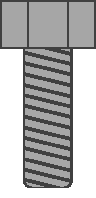
\includegraphics[width=6mm]{images/register-2.pdf}};
\end{tikzpicture}%
\hspace{3mm}
\begin{tikzpicture}
    \draw                    (0mm,0mm) -- (0mm,16mm) -- (22mm,16mm) -- (22mm,0mm) -- (0mm,0mm);
    \draw[very thin, dashed] (-0.5mm,-0.5mm) -- (-0.5mm,16.5mm) -- (22.5mm,16.5mm) -- (22.5mm,-0.5mm) -- (-0.5mm,-0.5mm);
    \draw[very thin]         (0mm,8mm) -- (22mm,8mm);
    \node[align=center]   at (11mm,4mm) {\footnotesize\circled{3} Bolzen};
    \node[align=center, rotate=90] at (11mm,12mm) {
\includegraphics[width=6mm]{images/register-3.pdf}};
\end{tikzpicture}%
\hspace{3mm}
\begin{tikzpicture}
    \draw                    (0mm,0mm) -- (0mm,16mm) -- (22mm,16mm) -- (22mm,0mm) -- (0mm,0mm);
    \draw[very thin, dashed] (-0.5mm,-0.5mm) -- (-0.5mm,16.5mm) -- (22.5mm,16.5mm) -- (22.5mm,-0.5mm) -- (-0.5mm,-0.5mm);
    \draw[very thin]         (0mm,8mm) -- (22mm,8mm);
    \node[align=center]   at (11mm,4mm) {\footnotesize\circled{4} Augen};
    \node[align=center, rotate=90] at (11mm,12mm) {
\includegraphics[width=6mm]{images/register-4.pdf}};
\end{tikzpicture}%
\hspace{3mm}
\begin{tikzpicture}
    \draw                    (0mm,0mm) -- (0mm,16mm) -- (22mm,16mm) -- (22mm,0mm) -- (0mm,0mm);
    \draw[very thin, dashed] (-0.5mm,-0.5mm) -- (-0.5mm,16.5mm) -- (22.5mm,16.5mm) -- (22.5mm,-0.5mm) -- (-0.5mm,-0.5mm);
    \draw[very thin]         (0mm,8mm) -- (22mm,8mm);
    \node[align=center]   at (11mm,4mm) {\footnotesize\circled{5} Federn};
    \node[align=center, rotate=90] at (11mm,12mm) {
\includegraphics[width=6mm]{images/register-5.pdf}};
\end{tikzpicture}%
\hspace{3mm}
\begin{tikzpicture}
    \draw                    (0mm,0mm) -- (0mm,16mm) -- (22mm,16mm) -- (22mm,0mm) -- (0mm,0mm);
    \draw[very thin, dashed] (-0.5mm,-0.5mm) -- (-0.5mm,16.5mm) -- (22.5mm,16.5mm) -- (22.5mm,-0.5mm) -- (-0.5mm,-0.5mm);
    \draw[very thin]         (0mm,8mm) -- (22mm,8mm);
    \node[align=center]   at (11mm,4mm) {\footnotesize\circled{6} Kleben};
    \node[align=center, rotate=90] at (11mm,12mm) {
\includegraphics[width=6mm]{images/register-6.pdf}};
\end{tikzpicture}%
\\ \vspace{4mm}
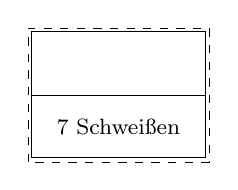
\begin{tikzpicture}
    \draw                    (0mm,0mm) -- (0mm,16mm) -- (22mm,16mm) -- (22mm,0mm) -- (0mm,0mm);
    \draw[very thin, dashed] (-0.5mm,-0.5mm) -- (-0.5mm,16.5mm) -- (22.5mm,16.5mm) -- (22.5mm,-0.5mm) -- (-0.5mm,-0.5mm);
    \draw[very thin]         (0mm,8mm) -- (22mm,8mm);
    \node[align=center]   at (11mm,4mm) {\footnotesize\circled{7} Schweißen};
\end{tikzpicture}%
\hspace{3mm}
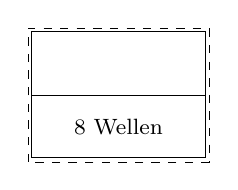
\begin{tikzpicture}
    \draw                    (0mm,0mm) -- (0mm,16mm) -- (22mm,16mm) -- (22mm,0mm) -- (0mm,0mm);
    \draw[very thin, dashed] (-0.5mm,-0.5mm) -- (-0.5mm,16.5mm) -- (22.5mm,16.5mm) -- (22.5mm,-0.5mm) -- (-0.5mm,-0.5mm);
    \draw[very thin]         (0mm,8mm) -- (22mm,8mm);
    \node[align=center]   at (11mm,4mm) {\footnotesize\circled{8} Wellen};
\end{tikzpicture}%
\hspace{3mm}
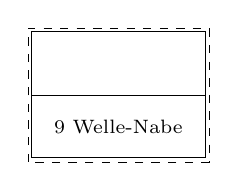
\begin{tikzpicture}
    \draw                    (0mm,0mm) -- (0mm,16mm) -- (22mm,16mm) -- (22mm,0mm) -- (0mm,0mm);
    \draw[very thin, dashed] (-0.5mm,-0.5mm) -- (-0.5mm,16.5mm) -- (22.5mm,16.5mm) -- (22.5mm,-0.5mm) -- (-0.5mm,-0.5mm);
    \draw[very thin]         (0mm,8mm) -- (22mm,8mm);
    \node[align=center]   at (11mm,4mm) {\scriptsize\circled{9} Welle-Nabe};
\end{tikzpicture}%
\hspace{3mm}
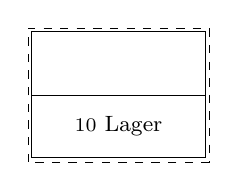
\begin{tikzpicture}
    \draw                    (0mm,0mm) -- (0mm,16mm) -- (22mm,16mm) -- (22mm,0mm) -- (0mm,0mm);
    \draw[very thin, dashed] (-0.5mm,-0.5mm) -- (-0.5mm,16.5mm) -- (22.5mm,16.5mm) -- (22.5mm,-0.5mm) -- (-0.5mm,-0.5mm);
    \draw[very thin]         (0mm,8mm) -- (22mm,8mm);
    \node[align=center]   at (11mm,4mm) {\footnotesize\circled{\scriptsize 10} Lager};
\end{tikzpicture}%
\hspace{3mm}
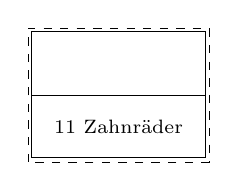
\begin{tikzpicture}
    \draw                    (0mm,0mm) -- (0mm,16mm) -- (22mm,16mm) -- (22mm,0mm) -- (0mm,0mm);
    \draw[very thin, dashed] (-0.5mm,-0.5mm) -- (-0.5mm,16.5mm) -- (22.5mm,16.5mm) -- (22.5mm,-0.5mm) -- (-0.5mm,-0.5mm);
    \draw[very thin]         (0mm,8mm) -- (22mm,8mm);
    \node[align=center]   at (11mm,4mm) {\footnotesize\scriptsize\circled{11} Zahnräder};
\end{tikzpicture}%
\hspace{3mm}
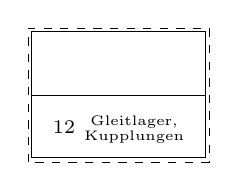
\begin{tikzpicture}
    \draw                    (0mm,0mm) -- (0mm,16mm) -- (22mm,16mm) -- (22mm,0mm) -- (0mm,0mm);
    \draw[very thin, dashed] (-0.5mm,-0.5mm) -- (-0.5mm,16.5mm) -- (22.5mm,16.5mm) -- (22.5mm,-0.5mm) -- (-0.5mm,-0.5mm);
    \draw[very thin]         (0mm,8mm) -- (22mm,8mm);
    \node[align=center]   at (11mm,4mm) {\circled{\scriptsize 12}~\begin{tabular}[c]{@{}c@{}}\tiny Gleitlager,\\[-1.5ex] \tiny Kupplungen\end{tabular}};
\end{tikzpicture}%
\vspace{15mm}

\myul{\textbf{Schritt 2:} Seite Auswählen (Symbol oder Schrift)}\\ \vspace{3mm}
\begin{minipage}{0.20\textwidth}
    \centering
    \hspace{22mm}%
    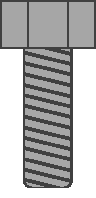
\includegraphics[width=7mm,angle=90]{images/register-2.pdf}
\end{minipage}%
\quad $\Longleftrightarrow$ \quad
\begin{minipage}{0.2\textwidth}
    $\left[\circled{2} \text{ Schrauben}\right]$
\end{minipage}
\\ \vspace{15mm}

\myul{\textbf{Schritt 3:} Register Aufkleben}\\ \vspace{4mm}\hspace{11mm}
\begin{tikzpicture}
    \draw[very thin] (0mm,0mm) -- (0mm,59.4mm) -- (42.0mm,59.4mm) -- (42.0mm,0mm) -- (0mm,0mm);             % Seite
    \draw[thin]      (42mm,52.8mm) -- (40.4mm,52.8mm) -- (40.4mm,57.2mm) -- (42mm,57.2mm);                  % Register-Platz
    \draw[->, rounded corners, thin] (49.5mm,29.7mm) -- (47mm,29.7mm) -- (47mm,55mm) -- (43.5mm,55mm);      % Pfeil
    \draw[thin]      (51mm,27.5mm) -- (51mm,31.9mm) -- (54.2mm,31.9mm) -- (54.2mm,27.5mm) -- (51mm,27.5mm); % Register
    \draw[very thin] (52.6mm,27.5mm) -- (52.6mm,31.9mm);                                                    % Register-Trenner
\end{tikzpicture}